\apendice{Especificación de diseño}

\section{Introducción}

El sistema completo funciona con la unión de dos subsistemas. El subsistema web, que lo forman el servidor que identifica al usuario, y la plataforma \textit{Jitsi}, para realizar la videollamada y el subsistema de colas, que da nombre a este trabajo, que encola los \textit{frames} del vídeo y los procesa. 

En este apartado se explica cómo se ha diseñado el sistema completo, la comunicación entre todas sus partes, el flujo del trabajo y la composición de cada elemento.

\section{Diseño procedimental}

El procedimiento para el procesado de los vídeos (\autoref{fig:secuencias}) para cada paciente que entre en una videollamada (independientemente de que esté o no el terapeuta) se inicializa un nuevo \texttt{Ingestor} que encolará los frames que reciba. A su vez este \texttt{Ingestor} creará un procesador que consumirá los \textit{frames} y los procesará. Estos dos elementos permanecerán hasta que sean cerrados por la finalización de la conexión. Por tanto, por cada paciente conectado se procesará tan pronto como sea posible la secuencia de \textit{frames} del mismo.

\begin{figure}
	\centering
	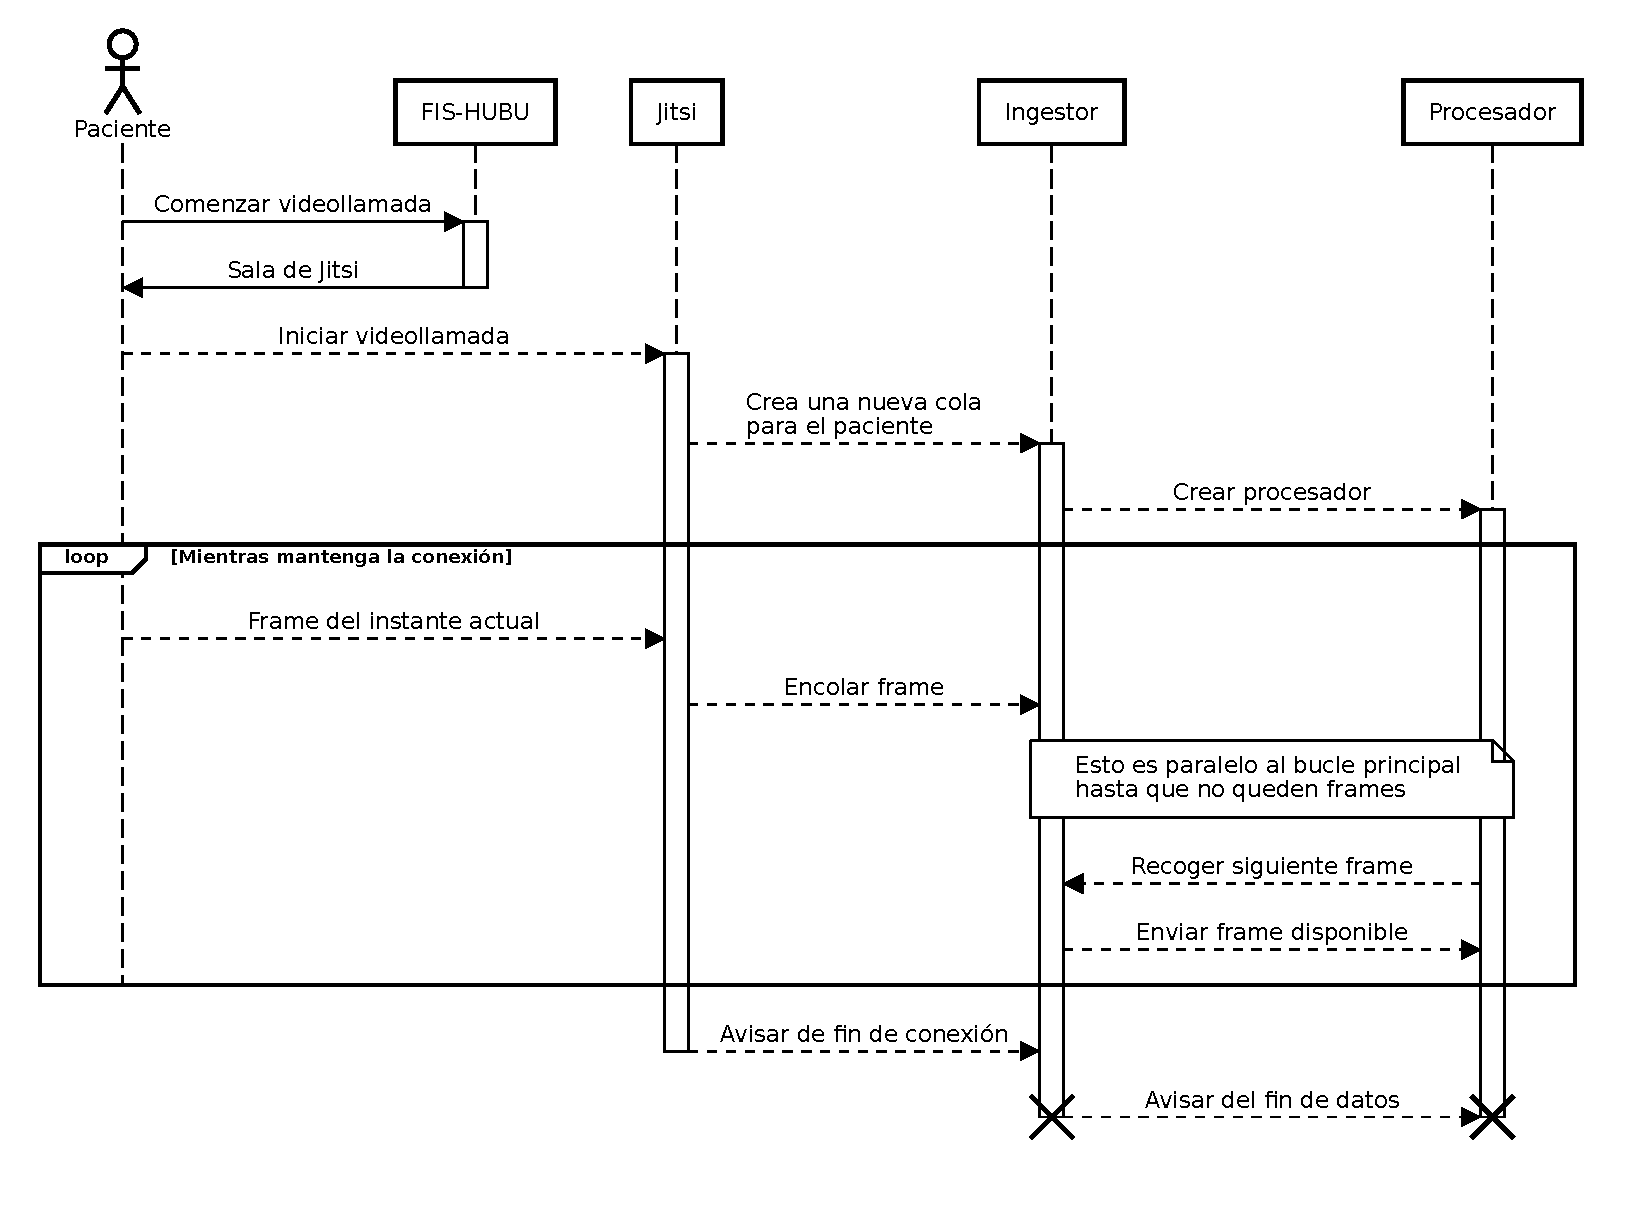
\includegraphics[width=\textwidth]{Secuencias}
	\caption[Diagrama de secuencia para el proceso general de la aplicación.]{Diagrama de secuencias para el proceso general de la aplicación. Conexión del paciente y procesado del vídeo de entrada.}
	\label{fig:secuencias}
\end{figure}



\section{Diseño arquitectónico}

La parte más esencial de este trabajo es la creación del \textit{pipeline} que procesa en tiempo real los \textit{frames} de la comunicación del paciente. Todo ello se ha desarrollado, utilizando las herramientas de la suite de \textit{Apache}, \textit{Apache Kafka} para el \textit{ingestor}, \textit{Apache Spark Streaming} para el \textit{procesador}. En la \autoref{fig:flujoetlreal} se puede observar el funcionamiento completo del flujo y las partes que lo componen.

Para que esta arquitectura sea ajena al entorno, se encapsulan sobre máquinas virtuales \textit{Docker} de tal forma que se pueda desplegar en cualquier sitio. Concretamente hay cuatro tipos de imágenes \textit{Docker}. La primera se encarga de la serialización de los frames y lanzan el \textit{script} de \textit{Python} de encolado, esta máquina se crea y destruye a voluntad de las conexiones de los pacientes. La segunda y tercera imágenes son el servicio de \textit{Zookeeper} y de \textit{Kafka}. Estas imágenes no se duplican en caso de cambios en las conexiones, únicamente se crean o borran colas. Por último, la cuarta imagen es la transformación del flujo. Se crean o se destruyen según las conexiones de los pacientes y se parametrizan para que consuman un flujo concreto y hagan un procesamiento concreto. De esta manera, diferentes pacientes se podrían configurar para tener diferentes procesados permitiendo una mayor flexibilidad en el procesamiento.

\begin{figure}[H]
	\centering
	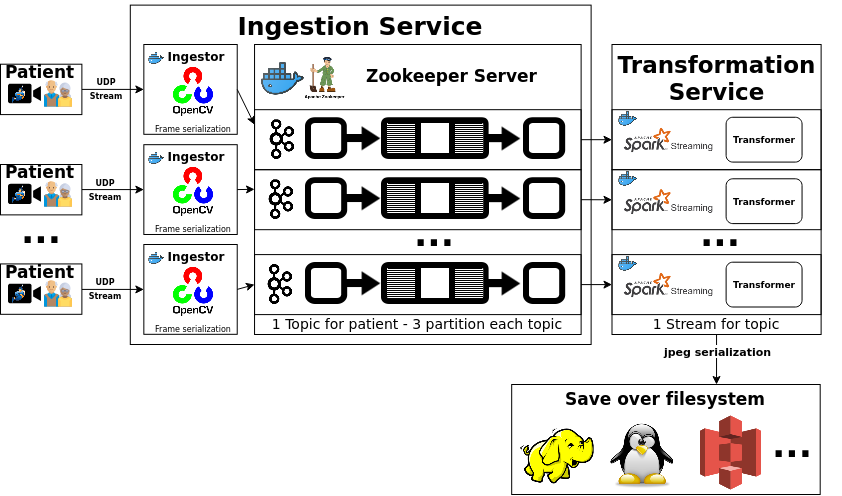
\includegraphics[width=\textwidth]{Flujo-FIS-HUBU}
	\caption[Implementación del flujo ETL para el procesado de imágenes en tiempo real.]{Implementación del flujo ETL para el procesado de imágenes en tiempo real. Por cada paciente conectado se asocia a un \textit{ingestor} que serializa la imagen y la encola en un flujo de \textit{Apache Kafka} dividido en tres particiones. Cada cola es procesada por un servidor de \textit{Apache Zookeeper}. El flujo es consumido por un procesador de \textit{Apache Spark Streaming}. El procesado puede ser cualquier operación con imágenes. Por último se almacena en el sistema de ficheros los resultados del flujo.}
	\label{fig:flujoetlreal}
\end{figure}

El diagrama de despliegue de las máquinas virtuales \textit{docker} se puede observar en la \autoref{fig:despligueDocker2}.

\begin{figure}
	\centering
	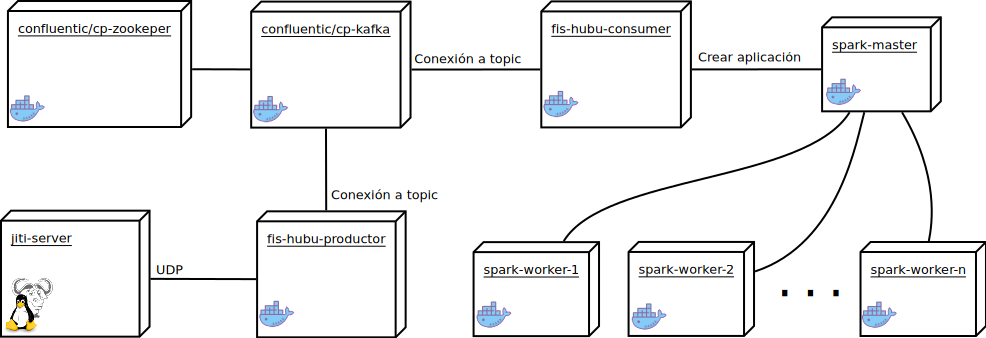
\includegraphics[width=1\textwidth]{img/DespliegueDocker.png}
	\caption{Diagrama de despliegue de las máquinas virtuales \textit{docker}.}
	\label{fig:despligueDocker2}
\end{figure}

